\documentclass[11pt,a4paper]{article}
\usepackage[utf8]{inputenc}
\usepackage[T1]{fontenc}
\usepackage[margin=1in,headheight=14pt]{geometry}
\usepackage{amsmath,amssymb,amsfonts}
\usepackage{booktabs,tabularx,array,listings,xcolor,hyperref,tikz,pgfplots,caption,microtype,enumitem,fancyhdr,titlesec,float,tocloft}
\pgfplotsset{compat=1.18}
\usetikzlibrary{shapes.geometric,arrows.meta,positioning,calc}
\raggedbottom
\definecolor{primaryblue}{RGB}{20,60,110}
\definecolor{secondarygreen}{RGB}{35,110,75}
\definecolor{accentgold}{RGB}{185,135,20}
\definecolor{darkslate}{RGB}{35,33,30}
\definecolor{lightgraybg}{RGB}{248,249,250}
\definecolor{bordergray}{RGB}{210,215,220}
\definecolor{commentgreen}{RGB}{34,139,34}
\definecolor{keywordblue}{RGB}{0,50,180}
\definecolor{stringred}{RGB}{175,35,35}
\hypersetup{colorlinks=true,linkcolor=primaryblue,citecolor=secondarygreen,urlcolor=primaryblue,pdftitle={Mockfish: An Intelligent Knowledge-Guided Adversarial Chess Engine},pdfauthor={Team Mockfish}}
\newcolumntype{L}[1]{>{\raggedright\arraybackslash}p{#1}}
\newcolumntype{C}[1]{>{\centering\arraybackslash}p{#1}}
\newcolumntype{R}[1]{>{\raggedleft\arraybackslash}p{#1}}
\newcolumntype{Y}{>{\raggedright\arraybackslash}X}
\titleformat{\section}{\normalfont\Large\bfseries\color{primaryblue}}{\thesection}{1em}{}[{\titlerule[0.8pt]}]
\titleformat{\subsection}{\normalfont\large\bfseries\color{darkslate}}{\thesubsection}{1em}{}
\titleformat{\subsubsection}{\normalfont\normalsize\bfseries\color{secondarygreen}}{\thesubsubsection}{1em}{}
\lstset{backgroundcolor=\color{lightgraybg},commentstyle=\color{commentgreen}\itshape,keywordstyle=\color{keywordblue}\bfseries,stringstyle=\color{stringred},basicstyle=\ttfamily\footnotesize,breaklines=true,captionpos=b,frame=single,rulecolor=\color{bordergray},numbers=left,numberstyle=\tiny\color{gray},numbersep=7pt,tabsize=4,showstringspaces=false}
\pagestyle{fancy}
\fancyhf{}
\fancyhead[L]{\small\color{gray}Mockfish: Knowledge-Guided Adversarial Chess Engine}
\fancyhead[R]{\small\color{gray}Introduction to AI with Python (25CS2000)}
\fancyfoot[C]{\thepage}
\renewcommand{\headrulewidth}{0.4pt}
\renewcommand{\footrulewidth}{0.4pt}
\begin{document}
\begin{titlepage}
    \centering
    \vspace*{1.5cm}
    {\Huge\bfseries\color{primaryblue} MOCKFISH \par}
    \vspace{0.4cm}
    {\LARGE\bfseries\color{darkslate} An Intelligent Knowledge-Guided Adversarial \\ Chess Engine \& Interactive GUI \par}
    \vspace{1.5cm}
    \colorbox{lightgraybg}{
        \begin{minipage}{0.88\textwidth}
        \vspace{0.35cm}
        \centering
        \renewcommand{\arraystretch}{1.45}
        \begin{tabular}{ll}
            \textbf{Course Name}: & Introduction to AI with Python \\
            \textbf{Course Code}: & 25CS2000 \\
            \textbf{GitHub Repository}: & \url{https://github.com/unclePRO/mockfish} \\
        \end{tabular}
        \vspace{0.35cm}
        \end{minipage}
    }
    \vspace{1.5cm}
    {\large\bfseries\color{primaryblue} Project Team Members \& System Allocations \par}
    \vspace{0.4cm}
    \renewcommand{\arraystretch}{1.35}
    \begin{tabularx}{0.96\textwidth}{l c Y l}
        \toprule
        \textbf{Student Name} & \textbf{Roll Number} & \textbf{Assigned Subsystem \& Role} & \textbf{Owned Module} \\
        \midrule
        \textbf{B Sreenikesh} & CS25B2051 & \textbf{Logic \& Rules Specialist}: Opening Book \& Knowledge-Based Rules & \texttt{knowledge\_base.py} \\
        \textbf{Aditya Kumar} & CS25I1050 & \textbf{State Space \& Heuristics}: Piece-Square Tables (PST) \& Eval & \texttt{heuristics.py} \\
        \textbf{Amit Kumar}   & CS25I1051 & \textbf{Adversarial Search}: Minimax, Alpha-Beta, Move Ordering & \texttt{search.py} \\
        \textbf{Aviral Pandey}& CS25B2054 & \textbf{GUI, Integrator \& Benchmark}: Canvas, Game Loop \& Metrics & \texttt{main.py}, \texttt{benchmark.py} \\
        \bottomrule
    \end{tabularx}
    \vfill
\end{titlepage}
\pagenumbering{roman}
\setcounter{page}{2}
\section*{Executive Summary}
\addcontentsline{toc}{section}{Executive Summary}
This report details the design, algorithmic formulation, empirical benchmarking, and architectural integration of \textbf{Mockfish}, an intelligent Python-based chess-playing application. Built to navigate the immense game tree of chess ($\sim 10^{120}$ theoretical variations), Mockfish synthesizes four core AI concepts: (1)~\textbf{Knowledge-Based Decision-Making} delivering expected $O(1)$ opening book lookups, (2)~\textbf{Adversarial Game Tree Search} utilizing Minimax with Alpha-Beta Pruning, (3)~\textbf{Tactical Move Ordering} prioritizing captures (MVV-LVA), pawn promotions, castling, and checks, and (4)~\textbf{State Space Evaluation} guided by simplified Piece-Square Tables (PST) and positional heuristics.

In the tactical exchange benchmark at depth~3, Alpha-Beta with heuristic move ordering achieved a \textbf{99.27\% reduction in visited nodes} relative to unpruned Minimax, reducing the estimated effective branching factor from $b_{eff}=37.35$ to $7.23$ and yielding a \textbf{141.74$\times$ execution speedup} ($0.16$ seconds versus $23.12$ seconds). The application provides an interactive 8$\times$8 Tkinter graphical interface with an in-canvas Game Over overlay that avoids blocking native result dialogs.
\vspace{0.4cm}
\hrule
\vspace{0.4cm}
% Keep the original contents styling, with compact section spacing to avoid a nearly empty page.
\setlength{\cftbeforesecskip}{3pt}
{\small\tableofcontents}
\newpage
\pagenumbering{arabic}
\setcounter{page}{1}
\section{Real-World Problem Identification \& Domain Relevance}
\subsection{Selected Domain: Intelligent Adversarial Game-Playing}
In fulfillment of coursework requirements, our four-member team selected the problem of constructing an \textbf{Intelligent Game-Playing Agent} for Chess. In artificial intelligence research, chess has historically served as a benchmark for evaluating how computational agents make sequential decisions under strict time constraints, adversarial pressure, and exponential state-space growth.
\subsection{Real-World Significance \& Transferability}
Although implemented as a classical board game, the underlying computational paradigms of Mockfish address fundamental challenges across diverse real-world domains:
\begin{enumerate}[leftmargin=*]
    \item \textbf{Adversarial Multi-Agent Environments}: In algorithmic automated trading, financial agents optimize portfolio capital in the presence of market makers and competitor algorithms attempting to exploit order books. Similarly, in autonomous cybersecurity response, defense agents continuously formulate counter-moves against dynamic network adversaries. Zero-sum minimax game trees provide formal optimality guarantees under worst-case assumptions.
    \item \textbf{Combinatorial Optimization \& Search Space Pruning}: With an estimated game-tree complexity of $10^{120}$ (the Shannon Number) and an average branching factor of $b \approx 35$, exhaustive search is impractical. Related branch-and-bound pruning and heuristic ordering principles can be applied to flight route scheduling, vehicle dispatching, and automated supply chain logistics.
    \item \textbf{Hybrid Decision Architectures}: Expert systems in clinical diagnostics and mission-critical industrial automation combine rule-based knowledge retrieval for standard protocols with dynamic heuristic search for rare, off-nominal events. Mockfish exemplifies this hybrid approach by pairing an expected $O(1)$ opening lookup with depth-limited adversarial search.
\end{enumerate}
\section{Formal Problem Formulation}
We formally formulate chess as a discrete, deterministic, turn-based, zero-sum, perfect-information adversarial environment defined by the 7-tuple:
\[\mathcal{M} = \langle S_0, Actions, Result, Constraints, Terminal\_Test, Utility, Heuristic \rangle\]
\begin{figure}[H]
\centering
\resizebox{0.96\textwidth}{!}{%
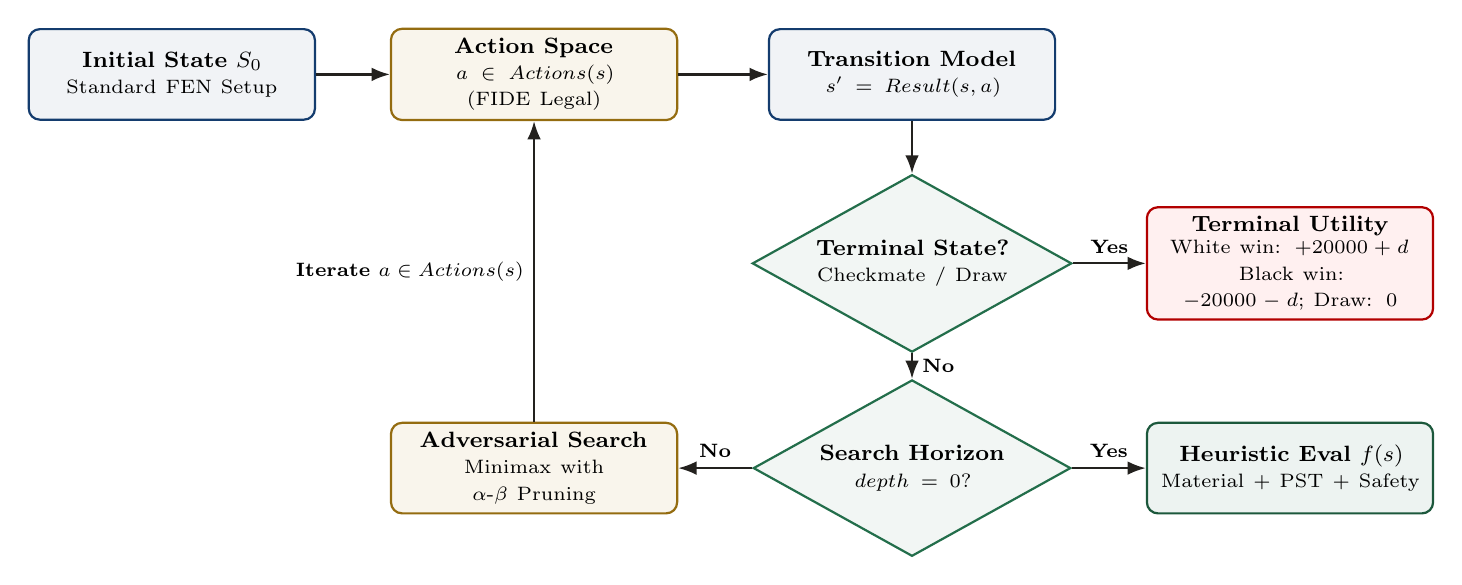
\begin{tikzpicture}[
    auto,
    block/.style={rectangle, draw=primaryblue, fill=primaryblue!6, text width=3.4cm, text centered, rounded corners=4pt, minimum height=1.15cm, font=\footnotesize\bfseries, thick},
    decision/.style={diamond, draw=secondarygreen, fill=secondarygreen!6, text width=2.6cm, text centered, inner sep=2pt, font=\footnotesize\bfseries, aspect=1.8, thick},
    action_block/.style={rectangle, draw=accentgold!80!black, fill=accentgold!8, text width=3.4cm, text centered, rounded corners=4pt, minimum height=1.15cm, font=\footnotesize\bfseries, thick},
    line/.style={draw=darkslate, -Latex, thick}]
    \node [block] (init) at (0, 0) {Initial State $S_0$\\ \normalfont\scriptsize Standard FEN Setup};
    \node [action_block] (act) at (4.6, 0) {Action Space\\ \normalfont\scriptsize $a\in Actions(s)$ (FIDE Legal)};
    \node [block] (trans) at (9.4, 0) {Transition Model\\ \normalfont\scriptsize $s' = Result(s, a)$};
    \node [decision] (term) at (9.4, -2.4) {Terminal State?\\ \normalfont\scriptsize Checkmate / Draw};
    \node [block, draw=red!70!black, fill=red!6] (util) at (14.2, -2.4) {Terminal Utility\\ \normalfont\scriptsize White win: $+20000+d$\\ Black win: $-20000-d$; Draw: $0$};
    \node [decision] (horizon) at (9.4, -5.0) {Search Horizon\\ \normalfont\scriptsize $depth = 0$?};
    \node [block, draw=secondarygreen!80!black, fill=secondarygreen!8] (heur) at (14.2, -5.0) {Heuristic Eval $f(s)$\\ \normalfont\scriptsize Material + PST + Safety};
    \node [action_block] (search) at (4.6, -5.0) {Adversarial Search\\ \normalfont\scriptsize Minimax with $\alpha$-$\beta$ Pruning};
    \path [line] (init) -- (act);
    \path [line] (act) -- (trans);
    \path [line] (trans) -- (term);
    \path [line] (term) -- node [above, font=\scriptsize\bfseries] {Yes} (util);
    \path [line] (term) -- node [right, font=\scriptsize\bfseries] {No} (horizon);
    \path [line] (horizon) -- node [above, font=\scriptsize\bfseries] {Yes} (heur);
    \path [line] (horizon) -- node [above, font=\scriptsize\bfseries] {No} (search);
    \path [line] (search) -- node [left, font=\scriptsize\bfseries] {Iterate $a \in Actions(s)$} (act);
\end{tikzpicture}}
\caption{Systemic Architecture and Problem Formulation Flowchart of Mockfish.}
\label{fig:problem_formulation}
\end{figure}
\subsection{Formal Component Definitions}
\begin{enumerate}[leftmargin=*]
    \item \textbf{Initial State ($S_0$)}: Standard 64-square layout formatted in Forsyth--Edwards Notation (FEN):
    \begin{center}
    \texttt{"rnbqkbnr/pppppppp/8/8/8/8/PPPPPPPP/RNBQKBNR w KQkq - 0 1"}
    \end{center}
    White to move, full castling rights ($\text{KQkq}$), zero half-move clock, move number 1.
    \item \textbf{State Space ($S$)}: The discrete set of legally reachable chess states, including piece placement, side to move, castling rights, en passant availability, move counters, and relevant move history for repetition. The number of legal board positions is commonly estimated to be on the order of $10^{40}$ or greater.
    \item \textbf{Action Space ($Actions(s)$)}: Legal moves are generated by \texttt{python-chess}: $\{m_1, m_2, \dots, m_k\}$ under FIDE rules, including pawn pushes/captures and special actions (Castling, En Passant, Promotions).
    \item \textbf{Transition Function ($Result(s,a)$)}: Deterministic state transition mapping current state $s$ and legal action $a \in Actions(s)$ to successor state $s'$. This toggles active color, updates piece bitboards, move counters, en passant availability, and castling rights.
    \item \textbf{Constraints ($C$)}:
    \begin{itemize}
        \item \textit{King Safety Constraint}: No player may execute an action that leaves their own king under attack:
        \[\forall a \in Actions(s),\quad \text{IsCheck}(Result(s,a),\text{Turn}(s))=\text{False}\]
        \item \textit{Check Evasion Constraint}: When in check, $Actions(s)$ is restricted to legal evasions that capture the attacking piece, interpose a defender, or move the king out of threat.
    \end{itemize}
    \item \textbf{Terminal Test \& Utility Function ($Utility(s,d)$)}:
    \[Utility(s,d)=\begin{cases}
    +20,000+d & \text{if Black is checkmated (White wins)}\\
    -20,000-d & \text{if White is checkmated (Black wins)}\\
    0 & \text{if the position is treated as a draw}
    \end{cases}\]
    Remaining depth $d$ rewards faster mates and delays forced losses. Game draws include stalemate, insufficient material and claimable draws. The search additionally treats twofold repetition as a zero-score cutoff to discourage shuffling; twofold repetition alone is not an official terminal draw.
    \item \textbf{Static Heuristic Evaluation ($f(s)$)}: Evaluated from White's perspective at the search horizon ($d=0$):
    \[f(s)=\Delta\text{Material}(s)+\Delta\text{PST}(s)+\Delta\text{Castling}(s)+\Delta\text{Rooks}(s)+\Delta\text{Bishops}(s)\]
\end{enumerate}
\noindent\textbf{Goal State:} Any legal position in which the opponent is checkmated. Because chess is adversarial, the agent seeks a win or the best achievable outcome against opposing moves; White maximizes utility and Black minimizes it.
\section{AI Algorithms Studied and Implemented}
Mockfish implements three principal search methods---depth-limited Minimax, Minimax with Alpha-Beta pruning, and Iterative Deepening---alongside knowledge-based retrieval, heuristic move ordering and static evaluation. Ordered Alpha-Beta is used in gameplay at a fixed depth of 3; the other search methods are implemented in \texttt{benchmark.py} for comparison.
\subsection{Knowledge-Based Opening System (\texttt{knowledge\_base.py})}
The knowledge-based subsystem operates as a deterministic lookup system. It indexes 11 known positions from openings including Ruy Lopez, Italian Game, Sicilian Defense, Queen's Gambit Declined, English, and Reti:
\begin{itemize}[leftmargin=*]
    \item \textbf{Complexity}: Expected $O(1)$ dictionary lookup time, $O(M)$ memory storage for $M$ cataloged positions (excluding FEN creation and move validation).
    \item \textbf{Functional Behavior}: If the board's FEN matches a known position, the engine returns the stored legal move without searching a game tree; otherwise it falls back to adversarial search. Formal logic inference and endgame tablebases are possible extensions, not current implementations.
\end{itemize}
\subsection{Algorithm 1: Exhaustive Minimax Search (Baseline Benchmark)}
Minimax assumes both players act with optimal adversarial rationality. With remaining depth $d$, its recurrence is:
\[V(s,d)=\begin{cases}
Utility(s,d) & \text{if } Terminal(s)\\
f(s)&\text{if }d=0\\
\max_{a\in Actions(s)} V(Result(s,a),d-1)&\text{if }Turn(s)=\text{White}\\
\min_{a\in Actions(s)} V(Result(s,a),d-1)&\text{if }Turn(s)=\text{Black}
\end{cases}\]
Because depth-limited exhaustive Minimax traverses up to $O(b^d)$ nodes in the tree, computational costs grow rapidly with depth.
\subsection{Algorithm 2: Minimax with Alpha-Beta Pruning (\texttt{search.py})}
Alpha-Beta pruning introduces dynamic branch-and-bound cutoffs using two threshold parameters:
\begin{itemize}[leftmargin=*]
    \item $\alpha$: The best lower bound established for the maximizing player.
    \item $\beta$: The best upper bound established for the minimizing player.
\end{itemize}
Whenever $\beta\le\alpha$, a cutoff occurs. Under identical terminal conditions and evaluation functions, Alpha-Beta preserves the depth-limited Minimax value. Its time complexity ranges from $O(b^{d/2})$ with ideal ordering to $O(b^d)$ in the worst case, with depth-first storage of $O(bd)$ for generated move lists. Root tie-breaking verifies potentially equal cutoff scores with a full-window search when preferring a non-repeating move.
\subsection{Heuristic Move Ordering (\texttt{search.py})}
The effectiveness of Alpha-Beta pruning depends critically on exploration order. If strong candidate moves are evaluated first, cutoffs can occur earlier. Mockfish implements a multi-tier heuristic move ordering policy:
\begin{enumerate}[leftmargin=*]
    \item \textbf{Captures via MVV-LVA}: Most Valuable Victim -- Least Valuable Attacker:
    \[\text{Priority}(m)=1000+100\cdot\text{Rank}(\text{Victim})-10\cdot\text{Rank}(\text{Attacker})\]
    The ranks are the library's piece-type identifiers, not material evaluation weights.
    \item \textbf{Pawn Promotions}: Queen promotions scored $+800$, Knight promotions $+500$, others $+200$.
    \item \textbf{Castling Moves}: Given $+300$ bonus to establish king safety early.
    \item \textbf{Direct Checks}: Moves delivering check receive $+150$.
    \item \textbf{Central Development}: Minor piece development to $\{d4,e4,d5,e5,c3,f3,c6,f6\}$ receives $+40$.
\end{enumerate}
\subsection{Algorithm 3: Iterative Deepening Search (\texttt{benchmark.py})}
Iterative Deepening Depth-First Search (IDDFS) repeatedly explores increasing depth limits while retaining the depth-first space complexity of $O(bd)$. In Mockfish, the benchmark applies ordered Alpha-Beta at depths $1,2,\dots,d_{max}$, retaining the best move from the latest completed iteration. The cost of repeated exhaustive depth-limited searches on a regular tree is $O(b^d)$ for fixed $b>1$; actual overhead with pruning depends on move ordering and position. This approach can support anytime search, but the current implementation stops at a predetermined maximum depth and does not enforce a time budget.
\subsection{State Space Heuristic Evaluation (\texttt{heuristics.py})}
The static evaluation function calculates granular positional features:
\begin{itemize}[leftmargin=*]
    \item \textbf{Material Base Weights}: Pawns ($1.00$), Knights ($3.20$), Bishops ($3.30$), Rooks ($5.00$), Queens ($9.00$).
    \item \textbf{Piece-Square Tables (PST)}: Map 64-square coordinates to positional values. For Black, coordinates are vertically mirrored via \texttt{square\_mirror(sq)}. Separate middlegame and endgame tables are used for the king.
    \item \textbf{Positional Factors}: Kingside/queenside castling rights ($+0.20/+0.15$), king placement on typical castled squares ($+0.35$), open/semi-open rook files ($+0.25/+0.15$), seventh-rank rooks ($+0.30$), and bishop pairs ($+0.30$).
\end{itemize}
\section{Empirical Performance Metrics \& Comparative Benchmarks}
\subsection{Experimental Setup}
Empirical evaluations were conducted on an Windows platform using the standalone benchmark engine \texttt{benchmark.py}. Two positions were evaluated across search depths 1 through 3:
\begin{enumerate}[leftmargin=*]
    \item \textbf{Position A (Italian Game Middlegame)}:
    \begin{itemize}[leftmargin=1.5em]
        \item \textbf{FEN}: \texttt{r1bqk2r/pppp1ppp/2n2n2/2b1p3/2B1P3/} \\
              \hspace*{0.9cm}\texttt{2N2N2/PPPP1PPP/R1BQK2R b KQkq - 5 4}
        \item \textbf{State Complexity}: 36 legal candidate moves available.
    \end{itemize}
    \item \textbf{Position B (Tactical Exchange Complex)}:
    \begin{itemize}[leftmargin=1.5em]
        \item \textbf{FEN}: \texttt{r1b1k2r/pppp1ppp/8/4N3/1b1nn3/} \\
              \hspace*{0.9cm}\texttt{2N5/PPPP1PPP/R1BQKB1R w KQkq - 0 7}
        \item \textbf{State Complexity}: 35 legal candidate moves available.
    \end{itemize}
\end{enumerate}
The metrics are visited search nodes (including internal nodes), elapsed wall-clock time measured using \texttt{time.perf\_counter()}, and an estimated effective branching factor $b_{eff}=N^{1/d}$, where $N$ is the reported node count. Table~\ref{tab:benchmark_results} reports the updated runs at all three depths for the tactical position and depth 3 for the Italian position.

\noindent\textbf{Methodological note:} All variants use the same static evaluation and terminal policy, including twofold repetition as a search cutoff. Each search counts its root; iterative deepening counts the root again at each depth. All four methods returned matching evaluation scores in all six position-depth combinations. Timings are single-run, position-specific observations and do not measure playing strength.
\subsection{Empirical Benchmark Results Table}
\begin{table}[H]
\centering
\caption{Empirical Benchmark Metrics Across Search Algorithms and Depths.}
\label{tab:benchmark_results}
\small
\renewcommand{\arraystretch}{1.2}
\begin{tabularx}{\textwidth}{@{} L{2.5cm} Y C{1.12cm} R{1.6cm} R{1.6cm} R{1.6cm} @{}}
\toprule
\textbf{Test Position} & \textbf{Algorithm} & \textbf{Depth} & \textbf{Nodes} & \textbf{Time (ms)} & \textbf{Est. $b_{eff}$} \\
\midrule
\textbf{Tactical} & Pure Minimax (Exhaustive) & 1 & 36 & 18.13 & 36.00 \\
\textbf{Exchange} & Alpha-Beta (Unordered) & 1 & 36 & 18.95 & 36.00 \\
& \textbf{Alpha-Beta + Move Ordering} & \textbf{1} & \textbf{36} & \textbf{20.33} & \textbf{36.00} \\
& Iterative Deepening (IDDFS) & 1 & 36 & 23.69 & 36.00 \\
\cmidrule{2-6}
& Pure Minimax (Exhaustive) & 2 & 1,555 & 589.20 & 39.43 \\
& Alpha-Beta (Unordered) & 2 & 269 & 96.76 & 16.40 \\
& \textbf{Alpha-Beta + Move Ordering} & \textbf{2} & \textbf{107} & \textbf{41.49} & \textbf{10.34} \\
& Iterative Deepening (IDDFS) & 2 & 143 & 61.24 & 11.96 \\
\cmidrule{2-6}
& Pure Minimax (Exhaustive) & 3 & 52,088 & 23,122.83 & 37.35 \\
& Alpha-Beta (Unordered) & 3 & 3,253 & 1,322.00 & 14.82 \\
& \textbf{Alpha-Beta + Move Ordering} & \textbf{3} & \textbf{378} & \textbf{163.13} & \textbf{7.23} \\
& Iterative Deepening (IDDFS) & 3 & 521 & 203.70 & 8.05 \\
\midrule
\textbf{Italian Game} & Pure Minimax (Exhaustive) & 3 & 44,701 & 19,625.57 & 35.49 \\
& Alpha-Beta (Unordered) & 3 & 10,775 & 4,113.20 & 22.09 \\
& \textbf{Alpha-Beta + Move Ordering} & \textbf{3} & \textbf{2,475} & \textbf{1,024.08} & \textbf{13.53} \\
& Iterative Deepening (IDDFS) & 3 & 2,696 & 1,121.21 & 13.92 \\
\bottomrule
\end{tabularx}
\end{table}
\subsection{Quantitative Performance Findings}
\begin{enumerate}[leftmargin=*]
    \item \textbf{Reduction in Nodes Visited}: In the tactical exchange position at depth~3, pure Minimax visited $52,088$ nodes. Alpha-Beta with move ordering visited $378$, a \textbf{99.27\%} reduction relative to Minimax.
    \item \textbf{Wall-Clock Speedup}: Execution time dropped from $23.12$ seconds to $0.16$ seconds, demonstrating a \textbf{141.74$\times$ execution speedup}. In the Italian position, the corresponding reduction was $94.46\%$ in nodes and $19.16\times$ in execution time.
    \item \textbf{Branching Factor Reduction}: The estimated effective branching factor ($b_{eff}=N^{1/d}$) decreased from $37.35$ to $7.23$ in the tactical test. This is a proxy for search growth, not the exact branching factor of the tree. At depth 1, all methods visit equal numbers of nodes; move ordering adds overhead without pruning savings.
\end{enumerate}
\begin{figure}[H]
\centering
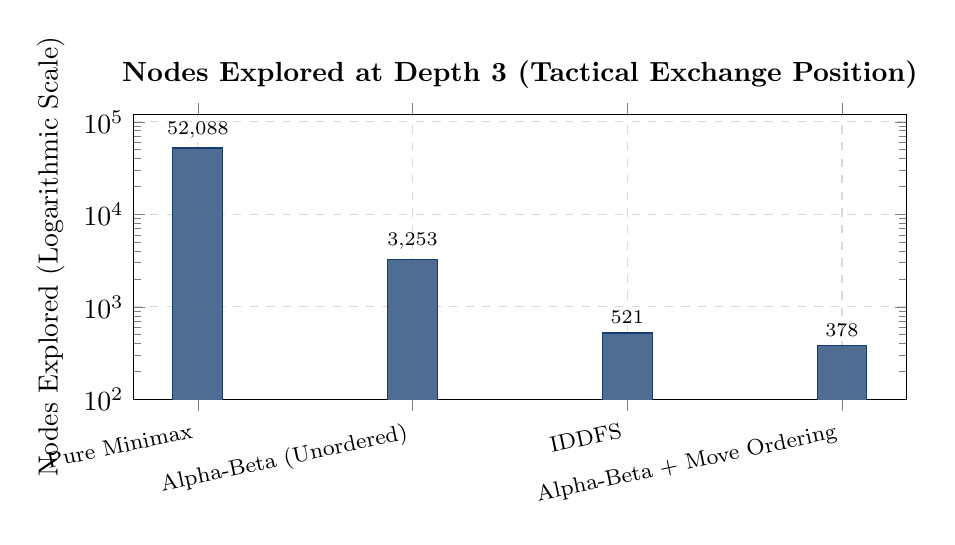
\begin{tikzpicture}
\begin{axis}[
    ybar,
    title={\textbf{Nodes Explored at Depth 3 (Tactical Exchange Position)}},
    ylabel={Nodes Explored (Logarithmic Scale)},
    symbolic x coords={PureMinimax, ABUnordered, IDDFS, ABMoveOrdering},
    xticklabels={Pure Minimax, {Alpha-Beta (Unordered)}, IDDFS, {Alpha-Beta + Move Ordering}},
    x tick label style={font=\footnotesize, rotate=12, anchor=north east},
    xtick=data,
    point meta=explicit symbolic,
    nodes near coords,
    nodes near coords style={font=\scriptsize},
    ymin=100, ymax=120000,
    ymode=log,
    bar width=18pt,
    width=0.94\textwidth,
    height=5.2cm,
    grid=major,
    grid style={dashed, gray!30}
]
\addplot[fill=primaryblue!75, draw=primaryblue] coordinates {
    (PureMinimax, 52088) [52,088]
    (ABUnordered, 3253) [3,253]
    (IDDFS, 521) [521]
    (ABMoveOrdering, 378) [378]
};
\end{axis}
\end{tikzpicture}
\caption{Empirical Node Count Comparison Across Algorithms at Depth 3.}
\label{fig:nodes_chart}
\end{figure}
\section{Justification: Method Selection Over Alternatives}
Course guidelines require justifying why Mockfish utilizes a \textbf{Hybrid Knowledge-Guided Alpha-Beta Search with Heuristic Evaluation} rather than other AI techniques:
\begin{table}[H]
\centering
\caption{Comparative Matrix: Why Mockfish Selected Alpha-Beta Over Other AI Methods.}
\label{tab:algorithm_justification}
\small
\renewcommand{\arraystretch}{1.2}
\begin{tabularx}{\textwidth}{@{} L{2.8cm} Y Y @{}}
\toprule
\textbf{Alternative AI Technique} & \textbf{Theoretical Capabilities} & \textbf{Justification for Rejection in This Domain} \\
\midrule
\textbf{Uninformed Search (BFS / DFS)} & BFS finds shortest paths in unweighted graphs; DFS explores deeply with lower memory usage. & BFS requires $O(b^d)$ memory in a depth-$d$ tree. Neither conventional method directly accounts for an adversary minimizing utility; DFS needs depth limits or cycle handling. \\
\textbf{A* / Greedy Best-First Search} & A* ranks $g(n)+h(n)$; Greedy uses $h(n)$ alone. & Standard versions target single-agent goal-directed search rather than alternating optimal adversarial decisions. \\
\textbf{Hill Climbing / Simulated Annealing} & Local search optimizing evaluation by greedy ascent or probabilistic downhill steps. & Vulnerable to local optima or plateaus; local evaluation alone does not model multi-ply opponent responses, e.g., a tempting capture followed by checkmate. \\
\textbf{Constraint Satisfaction (CSP / Backtracking)} & Solves discrete variable assignments satisfying static constraints. & Legal move generation involves constraints, but standard CSP formulations do not directly optimize adversarial utility. \\
\textbf{Deep Reinforcement Learning (AlphaZero)} & Neural policy/value networks trained via self-play. & Large-scale AlphaZero-style training requires substantial compute and implementation effort beyond this coursework's scope. \\
\midrule
\textbf{Mockfish Hybrid Approach (Alpha-Beta + PST)} & Branch-and-bound adversarial search coupled with expected $O(1)$ opening lookup and simplified PST heuristics. & Depth-limited adversarial decisions with $O(bd)$ search storage; recorded \textbf{141.74$\times$ speedup} and $99.27\%$ node reduction in the tactical depth-3 test; interpretable evaluation. \\
\bottomrule
\end{tabularx}
\end{table}
Ordered Alpha-Beta is preferred to unordered Alpha-Beta because the move-ordering heuristic substantially reduced the recorded node counts and runtime at depth 3 in both positions. Compared with iterative deepening to the same fixed maximum depth, the selected method avoids the repeated shallower searches; a time-limited iterative deepening engine may be useful in future work.
\section{Graphical User Interface \& System Architecture}
\subsection{Tkinter Canvas Architecture (\texttt{main.py})}
The GUI is implemented in Tkinter adhering to event-driven programming:
\begin{itemize}[leftmargin=*]
    \item \textbf{Visual Representation}: A 512$\times$512 canvas rendering high-contrast board squares (\texttt{\#EEEED2} warm cream and \texttt{\#769656} forest green) with dual-stroke Unicode pieces.
    \item \textbf{Move Guidance}: Clicking friendly pieces computes legal destinations dynamically, highlighting reachable empty squares with indicator dots and capturable enemy targets with hollow rings.
    \item \textbf{Dynamic Perspective}: Includes a \textit{Flip Board} feature that mirrors screen coordinates while preserving underlying chess logic coordinates.
    \item \textbf{Real-Time Telemetry HUD}: A dedicated status bar renders move UCI, source (opening book or search), and, for search moves, search depth, visited nodes and the search evaluation.
\end{itemize}
On the bot's turn, the GUI checks the opening book first and falls back to ordered Alpha-Beta at depth 3. The selected legal move is applied and the board and status bar are updated.
\subsection{Resolving Modal Dialog Blocking via Custom In-Canvas Overlay}
In early prototypes, invoking native OS modal dialogs (\texttt{messagebox.showinfo}) triggered event-loop blocking on Windows, making the window appear frozen upon checkmate.

We addressed this issue by developing an \textbf{in-canvas Game Over overlay card}:
\begin{itemize}[leftmargin=*]
    \item Rendered directly onto the canvas buffer without modal OS interruptions.
    \item Displays colored outcome banners (\textbf{WHITE WINS!}, \textbf{BLACK WINS!}, \textbf{DRAW!}), and specific termination reasons (\textit{Checkmate}, \textit{Stalemate}, \textit{Threefold Repetition}, \textit{50-Move Rule}).
    \item Features two interactive canvas buttons:
    \begin{itemize}
        \item \textbf{Play Again}: Resets board state, clears highlights, and begins a new match.
        \item \textbf{Review Board}: Dismisses the overlay card to allow post-game tactical inspection.
    \end{itemize}
    \item King check/checkmate states are highlighted directly on the board in warning red (\texttt{\#E53935}) and deep crimson (\texttt{\#B71C1C}).
\end{itemize}
The \texttt{root.after()} callback allows the human move to be rendered before search begins. Search itself runs on Tkinter's event thread, so this fix does not guarantee responsiveness during long searches.
\section{Team Member Contributions \& Collaborative Division}
To reduce merge conflicts during development, the codebase was partitioned into four modular layers:
\begin{table}[H]
\centering
\caption{Team Member Role Assignments and Detailed Technical Contributions.}
\label{tab:team_division}
\small
\renewcommand{\arraystretch}{1.25}
\begin{tabularx}{\textwidth}{@{} L{3.0cm} L{3.6cm} Y @{}}
\toprule
\textbf{Team Member} & \textbf{Assigned Module} & \textbf{Key Responsibilities \& Implemented Algorithms} \\
\midrule
\textbf{B Sreenikesh}\newline(CS25B2051) & Logic \& Rules Specialist (\texttt{knowledge\_base.py}) & Implemented opening book mapping for King's Pawn (\texttt{1. e4}), Queen's Pawn (\texttt{1. d4}), English, and Reti lines; FEN-based lookup, legality validation and fallback to adversarial search. \\
\addlinespace
\textbf{Aditya Kumar}\newline(CS25I1050) & State Space \& Heuristics (\texttt{heuristics.py}) & Implemented Piece-Square Tables (PST) with vertical reflection mirroring; formulated positional bonuses for castling, open rook files, and bishop pairs. \\
\addlinespace
\textbf{Amit Kumar}\newline(CS25I1051) & Adversarial Search Specialist (\texttt{search.py}) & Developed Minimax with Alpha-Beta pruning; engineered MVV-LVA move ordering, ply-adjusted checkmate scoring ($\pm(20000+d)$), and anti-shuffling repetition filters. \\
\addlinespace
\textbf{Aviral Pandey}\newline(CS25B2054) & GUI, Integrator \& Benchmarking (\texttt{main.py}, \texttt{test\_suite.py}, \texttt{benchmark.py}) & Developed Tkinter Canvas, in-canvas Game Over overlay card, board flipping, telemetry HUD, automated unit tests, and empirical benchmarking suite. \\
\bottomrule
\end{tabularx}
\end{table}
\subsection{Detailed Subsystem Breakdown by Member}
\begin{itemize}[leftmargin=*]
    \item \textbf{B Sreenikesh (CS25B2051 --- Logic \& Rules Specialist)}: Developed \texttt{knowledge\_base.py}. Formulated deterministic FEN pattern matching and indexed standard responses for $1.\,e4$, $1.\,d4$, $1.\,c4$, and $1.\,Nf3$. Implemented dictionary-based retrieval, move validation and fallback signaling.
    \item \textbf{Aditya Kumar (CS25I1050 --- State Space \& Heuristics Specialist)}: Developed \texttt{heuristics.py}. Formulated the multi-factor heuristic evaluation combining material base weights with Piece-Square Tables (PST), castling rights incentives ($+0.20/+0.15$), king placement bonus ($+0.35$), open-file rook bonuses ($+0.25$), and bishop pairs ($+0.30$).
    \item \textbf{Amit Kumar (CS25I1051 --- Adversarial Search Specialist)}: Developed \texttt{search.py}. Implemented Alpha-Beta pruning with ply-adjusted distance-to-mate scoring ($\pm(20000+d)$). Designed heuristic move ordering (MVV-LVA, promotions, checks, castling) and repetition filters to discourage rook shuffling.
    \item \textbf{Aviral Pandey (CS25B2054 --- GUI, Systems Integrator \& Benchmarking Specialist)}: Developed \texttt{main.py}, \texttt{benchmark.py}, and \texttt{test\_suite.py}. Built the 512$\times$512 Tkinter canvas interface, board flipping coordinate logic, and the custom in-canvas Game Over overlay card. Programmed the benchmark suite comparing execution times, estimated branching factors, and node traversal counts.
\end{itemize}
\section{Limitations \& Future Research Directions}
Ordered Alpha-Beta took approximately $0.16$--$1.02$\,s in the two reported depth-3 benchmarks. The live engine has fixed-depth search, a limited opening book and handcrafted evaluation.
\begin{enumerate}[leftmargin=*]
    \item \textbf{Quiescence Search (Horizon Effect Mitigation)}: At fixed depth 3, search may terminate immediately before an unresolved piece exchange. Extending tactical positions with quiescence search could mitigate the horizon effect.
    \item \textbf{Transposition Tables via Zobrist Hashing}: Identical board positions frequently recur via different move orders (transpositions). Caching evaluated subtrees in a hash-based table could reduce redundant evaluations; the improvement would need experimental validation.
    \item \textbf{Dynamic Time Management}: Allocating compute dynamically based on remaining clock time and positional volatility could allow deeper search in critical situations. A background worker could also improve GUI responsiveness during search.
    \item \textbf{Further Validation}: Root tie-breaking now re-searches ambiguous equal-score candidates when necessary, and search correctness tests passed for both tested positions. Additional positions, repeated timing trials and playing-strength evaluations would strengthen the empirical analysis.
\end{enumerate}
\section{Conclusion}
The \textbf{Mockfish} project successfully designed and implemented an intelligent, knowledge-guided adversarial chess engine in Python. By synthesizing a \textbf{Knowledge-Based Opening System} with \textbf{Alpha-Beta Pruning} and \textbf{Heuristic Move Ordering}, the project demonstrates the application of classical AI to chess:
\begin{itemize}[leftmargin=*]
    \item In the tactical exchange position at depth 3, reduced the estimated effective branching factor from $b_{eff}=37.35$ to $7.23$.
    \item Achieved a \textbf{99.27\% reduction in visited nodes} and a \textbf{141.74$\times$ execution speedup} ($0.16$\,s vs $23.12$\,s) in the same benchmark. In the Italian position, the recorded speedup was $19.16\times$.
    \item Addressed rook-shuffling behavior with repetition-aware heuristics and native modal dialog blocking with an in-canvas overlay interface.
    \item Passed all five test groups in \texttt{test\_suite.py}; all four benchmark configurations agreed on evaluation scores at each tested position and depth.
\end{itemize}
These results support the choice of ordered Alpha-Beta for fixed-depth gameplay in Mockfish. They demonstrate computational efficiency on the tested positions, not perfect play or universally guaranteed response times. Mockfish provides a functional demonstration of how classical Artificial Intelligence principles can be integrated into a practical application.
\begin{thebibliography}{9}
\bibitem{russell2020} S. Russell and P. Norvig, \textit{Artificial Intelligence: A Modern Approach}, 4th ed., Pearson, 2020.
\bibitem{knuth1975} D. E. Knuth and R. W. Moore, ``An analysis of alpha-beta pruning,'' \textit{Artificial Intelligence}, vol. 6, no. 4, pp. 293--326, 1975.
\bibitem{shannon1950} C. E. Shannon, ``Programming a computer for playing chess,'' \textit{Philosophical Magazine}, vol. 41, no. 314, pp. 256--275, 1950.
\bibitem{pst} T. Michniewski, ``Simplified Evaluation Function,'' Chess Programming Wiki. [Online]. Available: \url{https://www.chessprogramming.org/Simplified_Evaluation_Function}
\end{thebibliography}
\end{document}
